%----------------------------------------------------------------------------------------
%	PACKAGES AND DOCUMENT CONFIGURATIONS
%----------------------------------------------------------------------------------------
\documentclass[11pt]{article}
\usepackage{amsmath} % Required for some math elements
\usepackage{hyperref} 
\usepackage{xcolor}
\usepackage{lipsum} 
\usepackage{cite}
\usepackage{graphicx} % Required for the inclusion of images
\usepackage{algorithmic}
\usepackage{array}
\usepackage{bookmark}
\usepackage{listings}
\usepackage{amssymb}
\usepackage{enumitem}
\usepackage[margin=16mm]{geometry}
\usepackage[caption=false, font=footnotesize]{subfig}
\usepackage{fancyhdr}
\renewcommand{\headrulewidth}{0.4pt}
\renewcommand{\footrulewidth}{0.4pt}

\usepackage[active,tightpage]{preview}
\renewcommand{\PreviewBorder}{1in}
\newcommand{\Newpage}{\end{preview}\begin{preview}}

\newlist{steps}{enumerate}{1}
\setlist[steps, 1]{label = Step \arabic*:}

\hypersetup{ %color attributes of citation, link, etc.
    colorlinks=true,
    linkcolor=blue,
    filecolor=gray,      
    urlcolor=blue,
    citecolor=blue,
}

\newcommand{\matlab}{\textsc{Matlab }} %very important and totally necessary addition

\newcommand\Item[1][]{%
  \ifx\relax#1\relax  \item \else \item[#1] \fi
  \abovedisplayskip=0pt\abovedisplayshortskip=0pt~\vspace*{-\baselineskip}}
%----------------------------------------------------------------------------------------
%	DOCUMENT INFORMATION
%----------------------------------------------------------------------------------------

\title{ECEN 415 \\ Assignment 1 Submission}
\author{Daniel Eisen : 300447549}
\date{\today}

\begin{document}
\begin{preview}
\maketitle

%----------------------------------------------------------------------------------------
%	DOCUMENT CONTENT
%----------------------------------------------------------------------------------------
\section*{Section A - Formative Questions}
\begin{enumerate}
    \item 
    \begin{enumerate}
        \item 
        $$G_1(s) = \frac{20(s^2 + s + 0.5)}{s(s+1)(s+10)}$$
        \begin{center}
            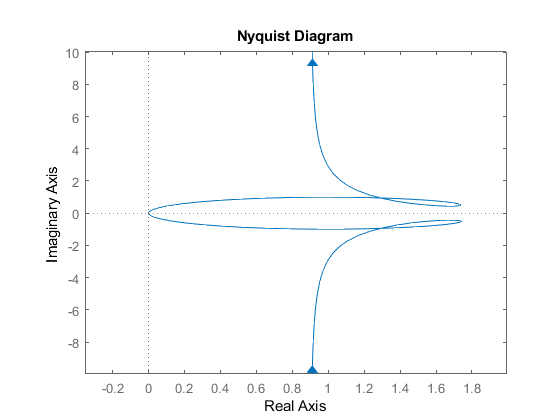
\includegraphics[width=0.33\textwidth]{fig/1a.png}
        \end{center}
        The system in its current state is stable as there are no enclosures of the critical point, and no open open-loop poles in the right half side of the s-plane. No level of gain from $0 \rightarrow \infty$ results in an enclosure, and thus the system cannot be made unstable with this method.  
        \item 
        $$G_2(s) = \frac{20(s^2 + s + 0.5)}{s(s-1)(s+10)}$$
        \begin{center}
            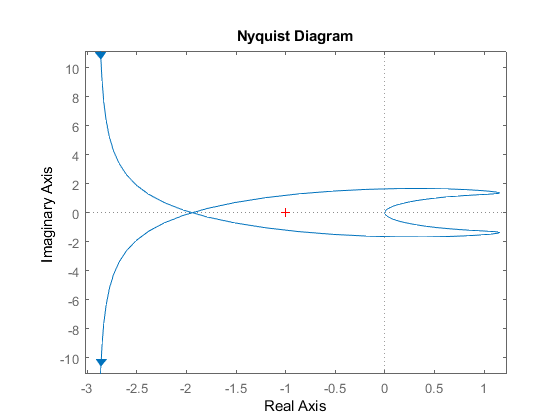
\includegraphics[width=0.33\textwidth]{fig/1b.png}
        \end{center}
        The system in its current state is stable as there is one open-loop pole in the right half side of the s-plane and one anti-clockwise encirclement of the critical point. However with reduced gain, there will be no enclosure of the critical point and the system can be driven unstable.
        \item 
        $$G_3(s) = \frac{s^2 + 3}{(s+1)^2}$$
        \begin{center}
            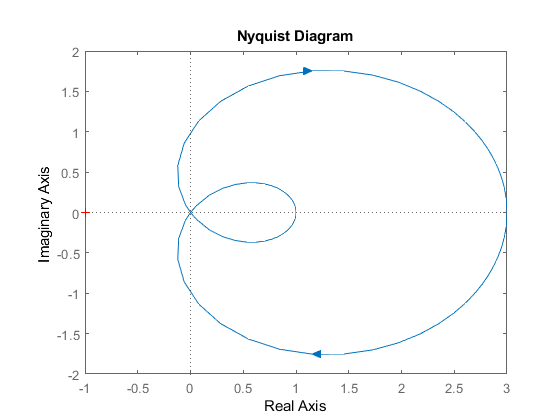
\includegraphics[width=0.33\textwidth]{fig/1c.png}
        \end{center}
        The system in its current state is stable as there are no enclosures of the critical point, and no open open-loop poles in the right half side of the s-plane.  No level of gain from $0 \rightarrow \infty$ results in an enclosure, and thus the system cannot be made unstable with this method.
        \item 
        $$G_4(s) = \frac{3(s+1)}{s(s-10)}$$
        \begin{center}
            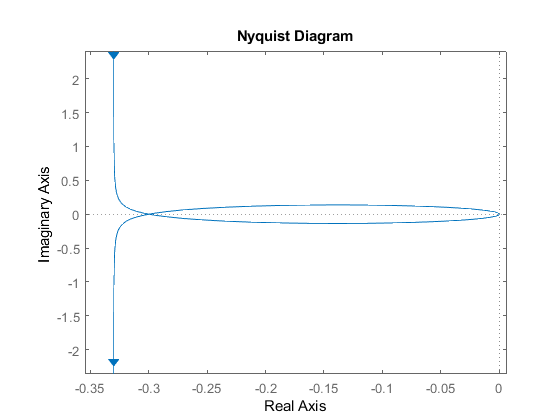
\includegraphics[width=0.33\textwidth]{fig/1d.png}
        \end{center}
        The system is currently unstable, as there is one open-loop pole in the right half side of the s-plane and no anti-clockwise encirclements of the critical point. By increasing the gain we can make and anti-clockwise encirclement of the critical point and result in a stable system.
    \end{enumerate}
    \item
    $$G = e^{-0.2s}\frac{4}{s+2}$$
    \begin{center}
        Eq: Delayed transfer function
    \end{center}
    \begin{enumerate}
        \item $\;$
        \begin{center}
            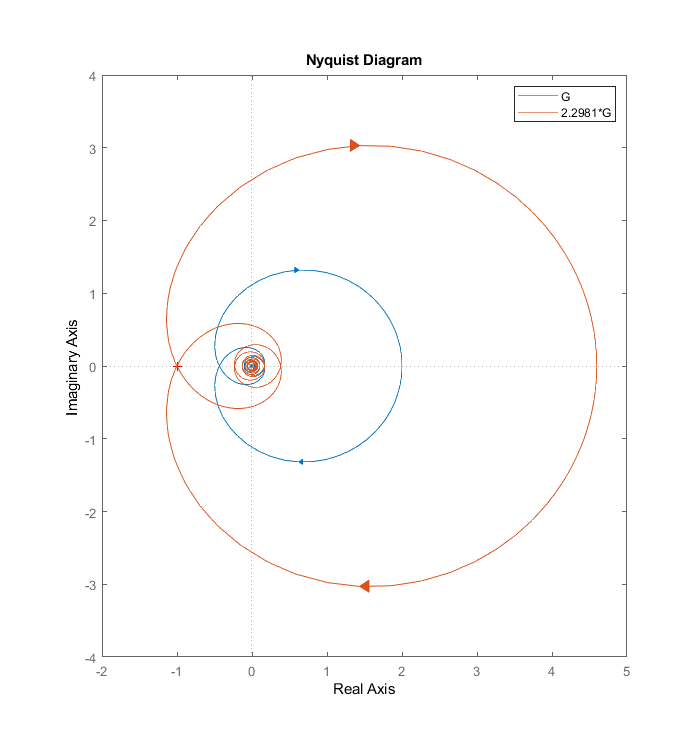
\includegraphics[width=0.33\textwidth]{fig/2a.png}
        \end{center}
        With no right hand poles and no critical enclosures the system is currently stable. Though with more gain the critical point can be enclosed and the system can be driven unstable. By extracting the gain margin from the system with \matlab we get a value of $2.2940$, the figure above show the original system and the system this the added gain, this shows the plot with a clockwise enclosure of -1 and thus the threshold on instabitly (via added gain).   
        \item $\;$
        \begin{center}
            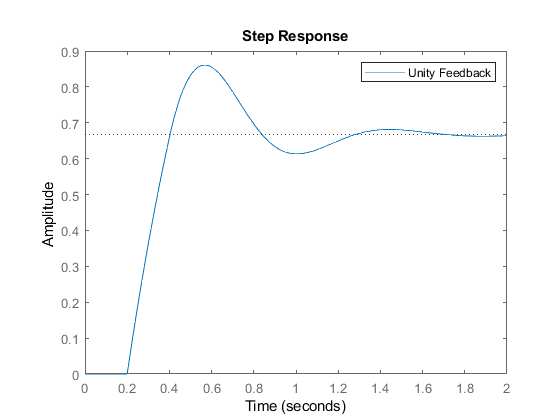
\includegraphics[height=0.33\textwidth]{fig/2bs.png}
            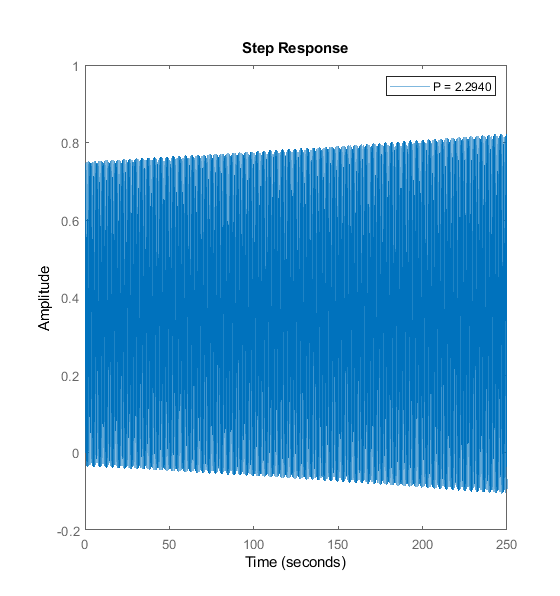
\includegraphics[height=0.33\textwidth]{fig/2bu.png}

            \textit{\hspace*{0.15\textwidth} Original System \hspace*{0.15\textwidth} Closed Loops gain from (a)}
        \end{center}
        Closing the loop with a proportional controller value of 2.2940 (as found in a) drives the system just into instabitly as predicted by inspecting the Nyquist plot.
        \item $\;$
        \begin{center}
            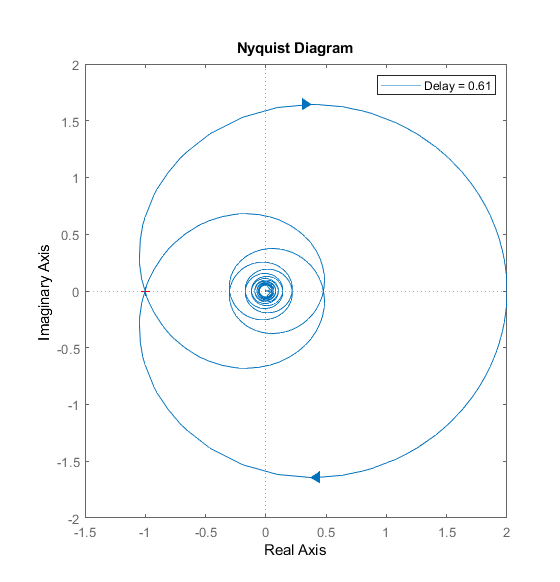
\includegraphics[width=0.33\textwidth]{fig/2c.png}
        \end{center}
        The figure above shows that a delay time of 0.61 causes the Nyquist plot to enclose the critical point. Though note a differences from the increased gain plot, smaller overall plot and a tighter enclosure divergence angle. 
    \end{enumerate} 
    \item $\;$
    \begin{center}
        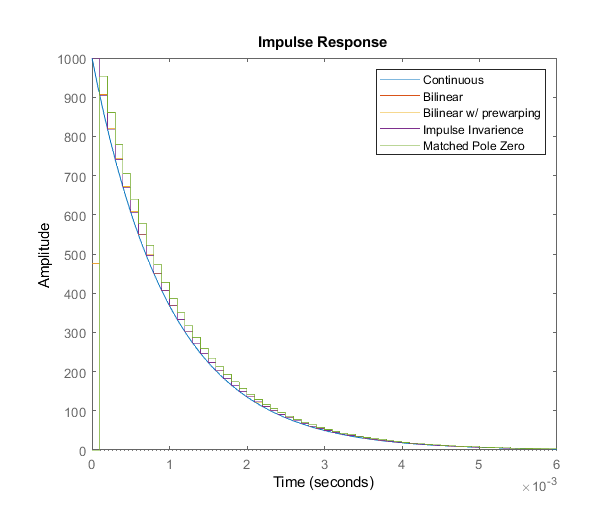
\includegraphics[height=0.25\textwidth]{fig/3_imp.png}
        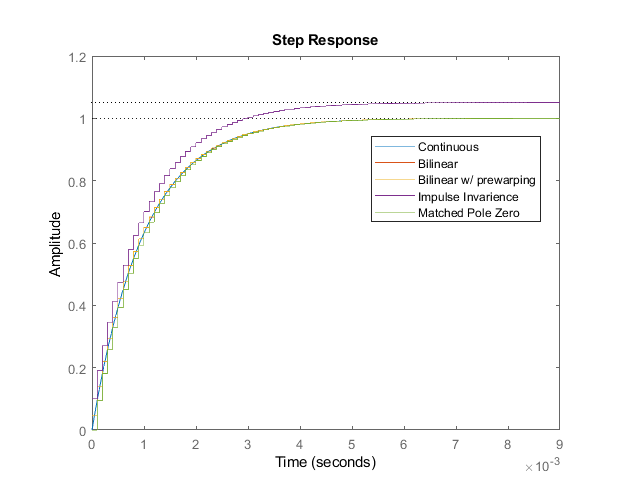
\includegraphics[height=0.25\textwidth]{fig/3_stp.png}
        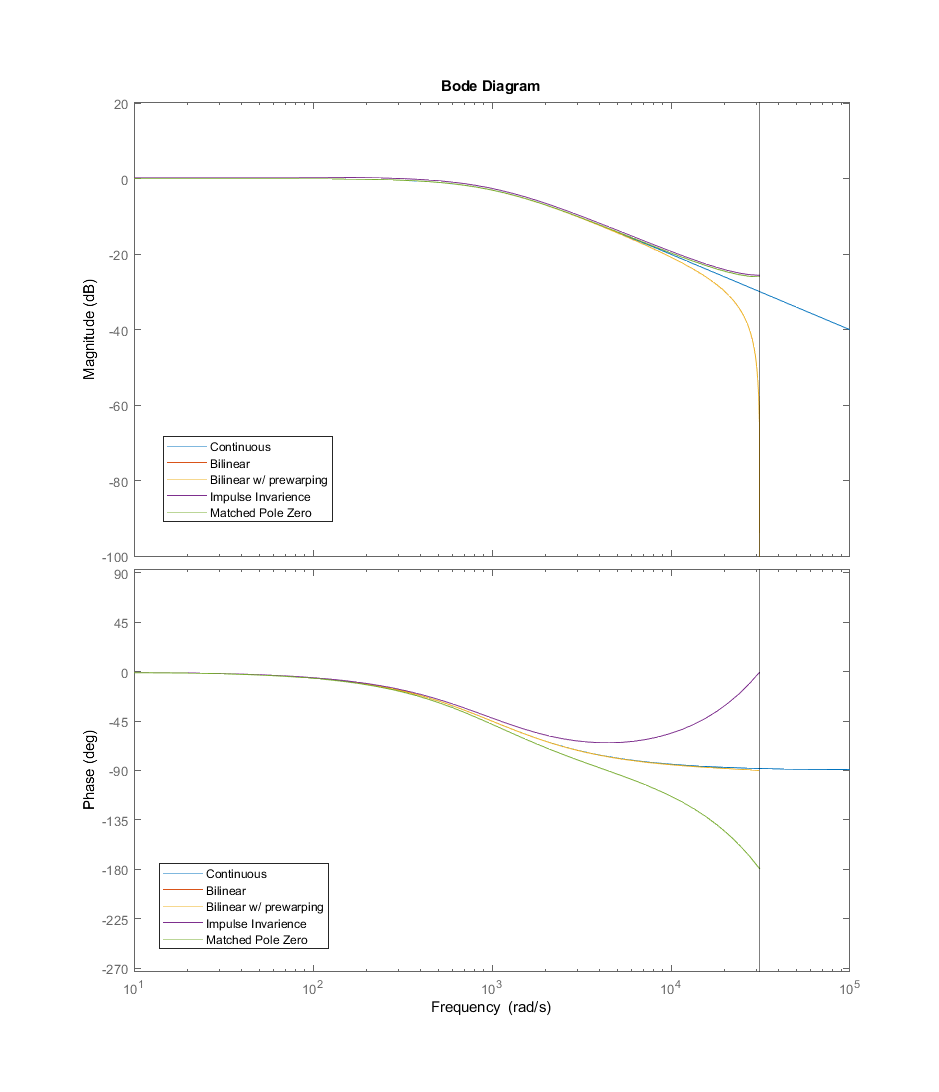
\includegraphics[height=0.25\textwidth]{fig/3_bode.png}
    \end{center}
    The above figure show the different conversion methods time and frequency responses. All but the impulse invariance method perform accurately to a step, which has steady state error. All perform well to an impulse but the impulse invariance is the only one to lack a delay delay at 0.

    Frequency response reveal larger differences in these methods. The bilinear methods by far more closely match the model system in phase and do not violate the gain roll of at higher frequencies like impulse invariance and match pole-zero, in fact increasing roll off. Also note the huge divergence from the model phase of both impulse and matched.
\end{enumerate}

\section*{Section B - Summative Questions}
\begin{enumerate}
    \item 
    \begin{enumerate}
        \item $$D(s)=e^{st_{d}} = e^{(\sigma+j\omega)t_{d}}$$
        $$e^{j\omega t_d} = cos(\omega t_d) + jsin(\omega t_d)$$
        $$\omega t_d = -\frac{\pi}{2},\; \omega = -\frac{\pi}{2t_d}$$
        \item $$\omega = 1000 rad/s, \; \phi=15^{\circ} = \frac{\pi}{12}$$
        $$t_d = \frac{\pi}{1200} \approx 0.00261799388$$
        \item Using \matlab to model the 1st and 2nd Pade approximations and modifying ts until $\phi=15^{\circ}$. 
            \begin{center}
                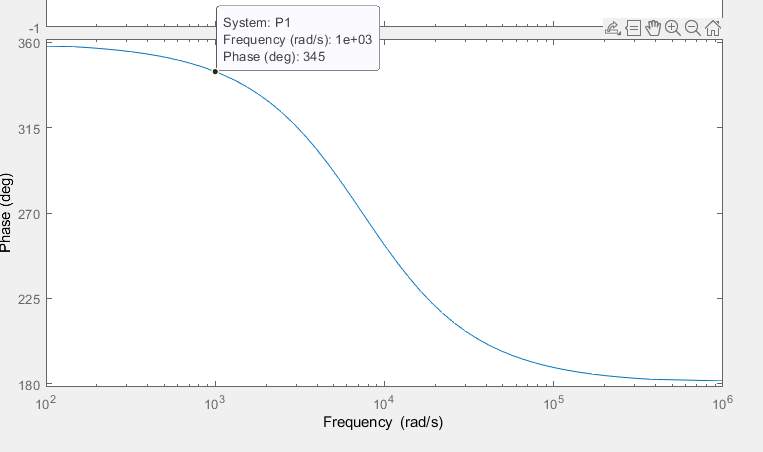
\includegraphics[width=0.3\textwidth]{fig/b1c_270u.png}
                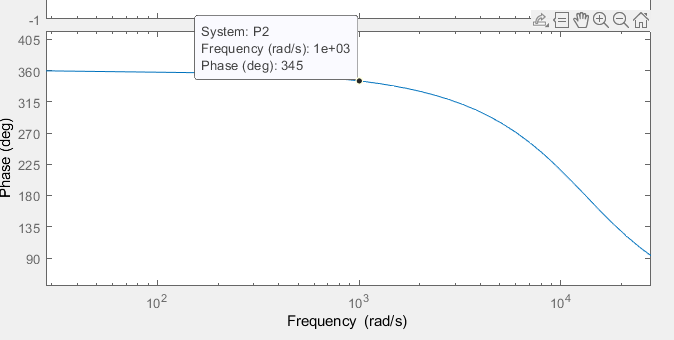
\includegraphics[width=0.3\textwidth]{fig/b1c_2_261u.png}

                \textit{1st Pade \hspace*{0.2\textwidth} 2nd Pade}
            \end{center}
            Figure above show the resultant gain of the frequency response of these approximations. This results in a ts 0.00027 for the 1st and 0.000261 for the 2nd. Both already close to the model delay.
    \end{enumerate}
    \item
    $$sampler = \frac{1-e^{st_s}}{s}$$
    $$pade: e^{st_s} \approx \frac{1-s\frac{t_2}{2}}{1+s\frac{t_s}{2}}$$
    $$substitute \rightarrow sampler \approx \frac{2}{s + \frac{s}{t_s}}$$
    \begin{center}
        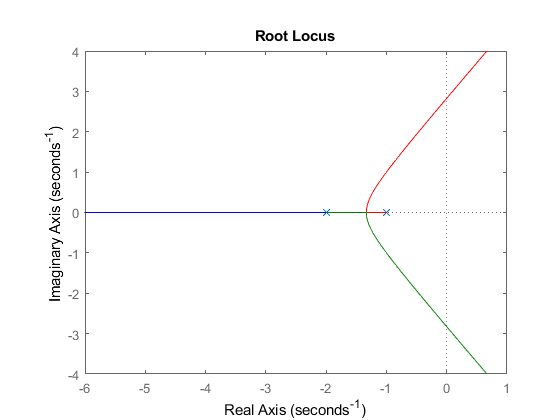
\includegraphics[width=0.25\textwidth]{fig/b2_ts_1_rloc.png}
        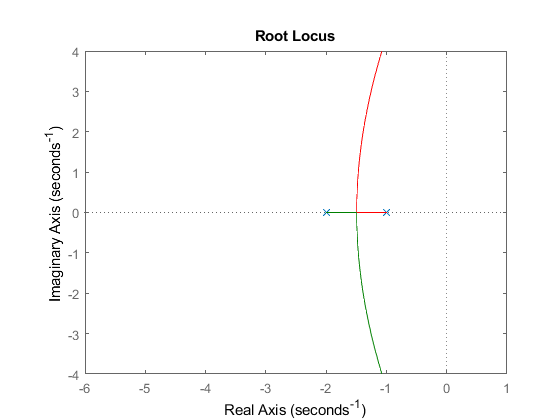
\includegraphics[width=0.25\textwidth]{fig/b2_ts_0.1_rloc.png}
        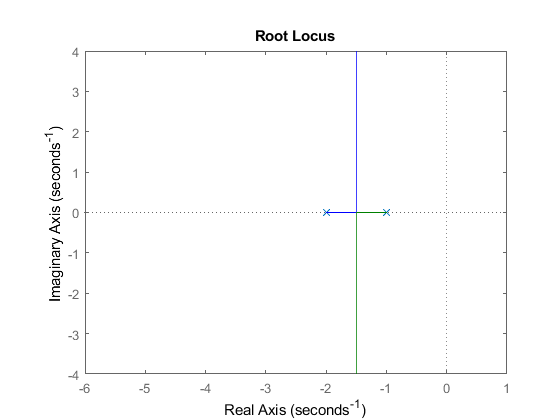
\includegraphics[width=0.25\textwidth]{fig/b2_cont_rloc.png}
    \end{center}
    Sampler inserts a left hand pole at 2/sampling time. Therefore as the sampling speed increases, the inserted pole becomes less and less dominant, the gain margin increases and the system more accurately represents the unsampled system. Figures above shows this progression with  (left to right) low sampling speed, higher sampling speed and unsampled system.

    For 10x: Unity gain frequency is $3.55 rad/s = 0.565Hz$, new sampling: $f = 5.56Hz, t_s = 0.177$
    \begin{center}
        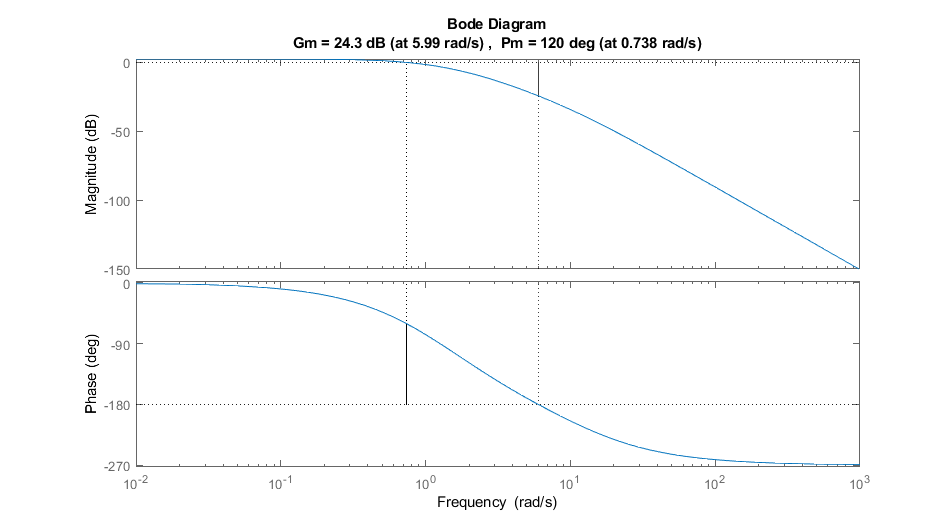
\includegraphics[width=0.5\textwidth]{fig/b2GM.png}
    \end{center}
    Resultant gain margin is 24.3dB (16.3590).
    \item 
    To minimise the sampling frequency, the corner frequency is set as a function of it. To satisfy the requirement of -40dB (per decade of 2nd order filter) attenuation of aliased signal the corner is set 1 decade before the nyquist frequency, ie fc = fs/20.

    At minimum, fs must be set to 100kHz (fc = 5kHz), but this exceeds the phase margin of the system (10 degrees.)

    In \matlab the sampling frequency is increased (retaining the fc relationship), and computing the phase at 10kHz of a sampled Butterworth filter until it reduced to 10 degrees.  

    $$fs = 1.81Mhz, fc = fs/20$$

    Though note the gain of the sampled system is heavily reduced so this would still need to the scaled.
    \begin{center}
        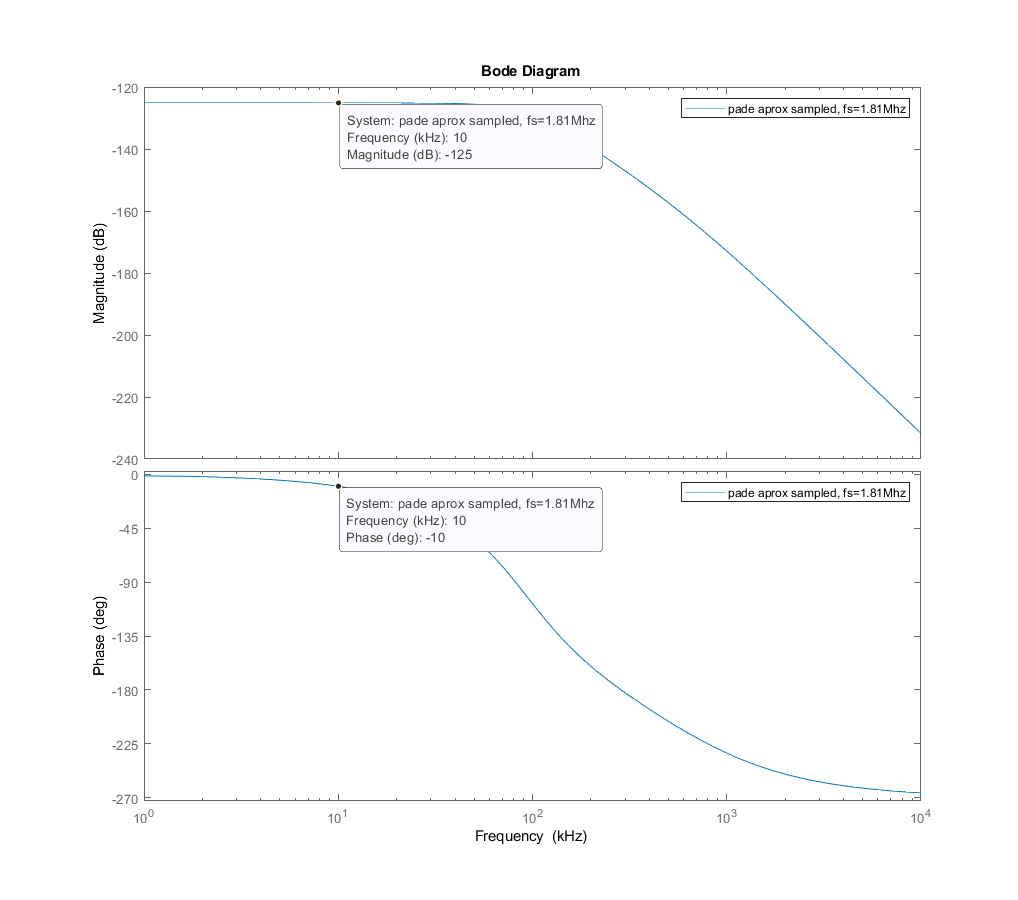
\includegraphics[width=0.3\textwidth]{fig/b3.png}

        \textit{Frequency Response (using 1st Pade delay)}
    \end{center}
\end{enumerate}
\end{preview}
\end{document}